\section{Radial Intensity drop off}
\label{sec:radial_intensity}
Due to the star in the center of the image, there is an intensity decrease in radial direction. This light coming from the star makes it harder to find other objects and structures close to it. Therefore we want to get rid of it. This is a lot easier in the $r$-$\varphi$ plane, where the intensity decrease is parallel to the $r$ axis as we can see in figure \ref{fig:warping_R150-300} b) and this drop-off can be described by an exponential decrease. In figure \ref{fig:mean_angular_intensity_R150_300} the mean angular intensity values are plotted against the radius and the data is fit by an exponential.
\begin{figure}[H]
	\centering
		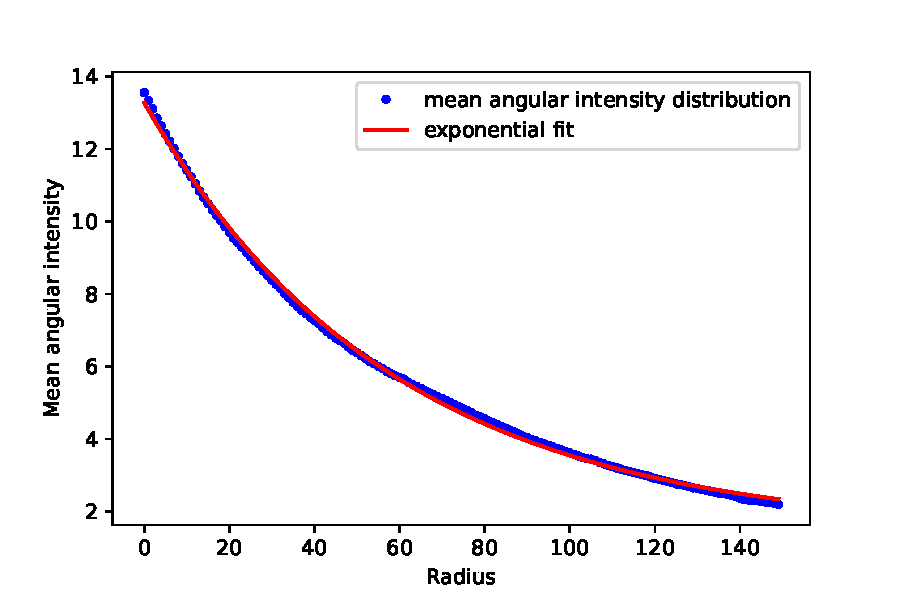
\includegraphics[width=0.9\textwidth]{pics/mean_angular_intensity_R150_300.pdf}
\caption{The intensity drop off due to the light from the star at radius zero can be described by an exponential fit.}
\label{fig:mean_angular_intensity_R150_300}
\end{figure}
The exponential fit describes the intensity drop off in a good way and by subtracting it from the $r$-$\varphi$ plane image we get an image where the mean intensity in radial direction is more or less constant. Figure \ref{fig:flatten_R150-300} shows the effect of this subtraction and we call the resulting image the flatten image.  
\begin{figure}[H]
	\centering
		\subfigure[]{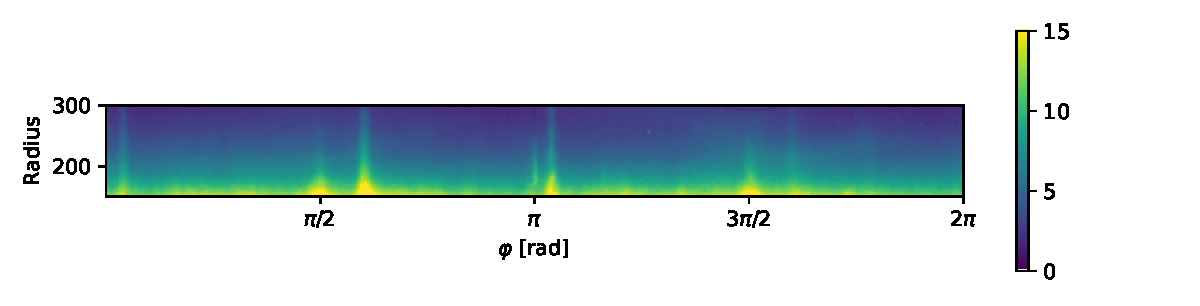
\includegraphics[width=1.0\textwidth]{pics/HDwarped_R150_R300_15.pdf}}
		\subfigure[]{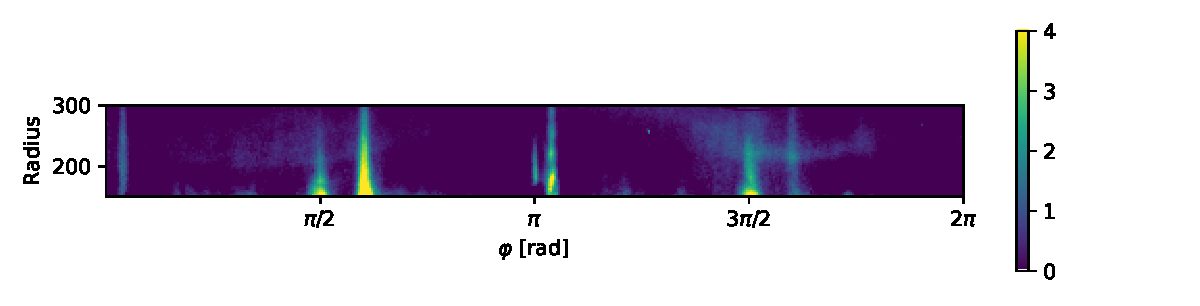
\includegraphics[width=1.0\textwidth]{pics/HDflatten_R150_R300_4.pdf}}
\caption{After the image transformation into the $r$-$\varphi$ plane (a), the image is flattened by subtracting the intensity which comes from the star at radius zero (b).}
\label{fig:flatten_R150-300}
\end{figure}
We insert a model planet (a faint copy of the star) into the image before the flattening of the image to make sure, that the aperture flux is not affected by the flattening. We find that the aperture flux change due to the flattening is only $0.03 \%$. So we can say that the aperture flux is not affected by this procedure. 